\documentclass[dcc, usedate]{fcfmcourse}
\usepackage{teoria}
\usepackage[utf8]{inputenc}
\usepackage[spanish]{babel}
\usepackage{epstopdf}
\usepackage{listings}
\usepackage{subcaption}

\usepackage{listings}
\usepackage{color}
 
\definecolor{codegreen}{rgb}{0,0.6,0}
\definecolor{codegray}{rgb}{0.5,0.5,0.5}
\definecolor{codepurple}{rgb}{0.7,0,0.82}
\definecolor{backcolour}{rgb}{0.95,0.95,0.92}
 
\lstdefinestyle{mystyle}{
	backgroundcolor=\color{backcolour},   
    commentstyle=\color{codegreen},
    keywordstyle=\color{codepurple},
    numberstyle=\tiny\color{codegray},
    stringstyle=\color{codepurple},
    basicstyle=\footnotesize,
    breakatwhitespace=false,         
    breaklines=true,                 
    captionpos=b,                    
    keepspaces=true,                 
    numbers=left,                    
    numbersep=5pt,                  
    showspaces=false,                
    showstringspaces=false,
    showtabs=false,                  
    tabsize=2
}
 
\lstset{language=Java, style=mystyle}

\title[5]{Comparación de Árboles Balanceados}
\course[CC3001]{Algoritmos y Estructuras de Datos}
\professor{Nelson Baloian}
\professor{Patricio Poblete}
\assistant{Manuel Cáceres}
\assistant{Sebastián Ferrada}
\assistant{Sergio Peñafiel}
% Si pasas el comando usedate a la clase, la fecha aparecerá bajo la lista de auxiliares.
% Puedes usar el formato de fecha por defecto de latex (y traducirla usando babel)
% o puedes escribir lo que quieras con el comando \date.
\date{Fecha de entrega: 5 de junio, 23:59 hrs}

\DeclareMathOperator{\lev}{lev}
\DeclareMathOperator{\altura}{altura}
\begin{document}
\maketitle

\section{Introducción}
Un árbol de búsqueda binaria (ABB) es una estructura de datos para guardar llaves y que permite realizar búsquedas eficientes sobre ellas. Su complejidad promedio en tiempos de búsqueda e inserción es $O(\log n)$. Sin embargo, es sabido que el ABB se puede degenerar a una lista enlazada si los elementos son insertados ordenadamente, lo que nos lleva a que el peor caso de búsqueda e insersión en ABB es $O(n)$.

Para enfrentar este problema, existen otro tipo de ABBs llamados \textit{balanceados} ya que se preocupan de que la cantidad de nodos en los subárboles izquierdo y derecho de cada nodo sea lo más similar posible, poniendo así un límite en la altura final del árbol y asegurando que el tiempo de búsqueda sea $O(\log n)$.

En esta tarea se considerarán dos tipos de árboles balanceados:
\begin{itemize}
	\item \textbf{AVL} un AVL es un ABB tal que cada vez que un nodo es insertado (según el algoritmo usual de un ABB), se revisa que la condición $|\altura{(n.izq)} - \altura{(n.der)}| <= 1$ para todos los nodos $n$ del árbol. Si la condición es violada por algún nodo, se restaura utilizando rotaciones simples y dobles.
	\item \textbf{Rojo-negro} un árbol rojo-negro es un ABB en el cual sus nodos tienen un bit extra de información, llamado el \textit{color}. Cualquier nodo insertado en el árbol es de color rojo. Tras la inserción, se revisa que las siguientes condiciones sean cumplidas:
	\begin{itemize}
		\item La raíz del árbol es negra
		\item Todas las hojas (punteros \texttt{null}) son negros
		\item Si un nodo es rojo, sus dos hijos deben ser negros
		\item Dado un nodo, todos los caminos desde él hasta las hojas tienen la misma cantidad de nodos negros
	\end{itemize}
\end{itemize}
En la figura \ref{fig:fig1} se pueden ver ejemplos de ambos tipos de árboles
\begin{figure}[h]
\begin{subfigure}{.5\textwidth}
  \centering
  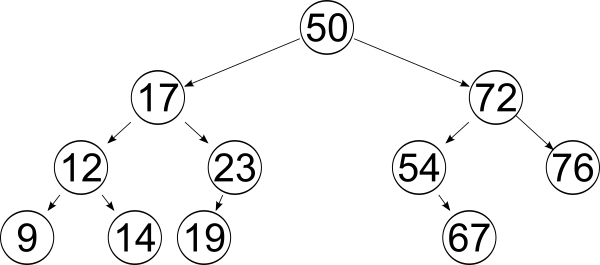
\includegraphics[width=.8\linewidth]{AVLtreef.png}
  \caption{AVL}
  \label{fig:sfig1}
\end{subfigure}%
\begin{subfigure}{.5\textwidth}
  \centering
  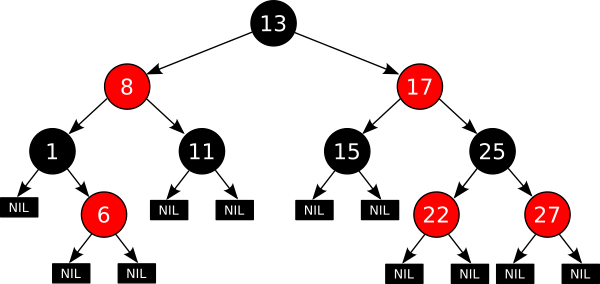
\includegraphics[width=.8\linewidth]{Red-black_tree_example.png}
  \caption{Rojo-negro}
  \label{fig:sfig2}
\end{subfigure}
\caption{Ejemplos de ABB}
\label{fig:fig1}
\end{figure}

\section{Implementación}
Su trabajo consistirá en implementar tres tipos de árboles: ABB normal, AVL y árbol rojo-negro. Para lo cual, se espera que entregue tres clases (una para cada árbol) que implementen la siguiente interfaz siguiendo las reglas mencionadas en la sección previa:
\begin{center}
\begin{lstlisting}
public interface ArbolBinario{
	public void insertar(int x);
	public boolean buscar(int x);
}
\end{lstlisting}
\end{center}

\section{Experimentación}
Una vez implementados los árboles, se le pide que los compare en diversos escenarios. Los indicadores a comparar deben ser definidos por usted, pero por ejemplo podría usar: la altura final del árbol, tiempo promedio de inserción/búsqueda, cantidad de nodos internos versus externos, etc.

Los escenarios son tuplas $(n, o)$ donde $n\in \{1000, 2000, ..., 10000\}$ es la cantidad de nodos a insertar y $o \in \{AZAR, ASC, OTRO\}$ la distribución de las llaves a insertar (al azar, números ordenados ascendentemente u otra inventada por ud. para forzar un comportamiento anómalo). Luego, si desea medir tiempos de búsqueda, puede realizar $1000$ o algún número que ud. considere significativo de búsquedas de elementos al azar en cada escenario.

Recuerde que si utiliza promedios, debe proveer la desviación estándar de los datos. Recuerte también que si está midiendo el tiempo de búsqueda, no puede realizar otras operaciones (como medir alturas o contar nodos visitados) simultáneamente, pues sus resultados estarán alterados.

Con los indicadores para los diferentes escenarios, realice gráficos que le ayuden a comparar la \textit{performance} de los distintos árboles. Pregúntese cuál es el peor caso para cada árbol (de existir alguno). ¿Cuál es la complejidad de la búsqueda? ¿Cuál árbol tiene mejor tiempo promedio? ¿Se ajustan a la cota $O(\log n)$?

\section{Condiciones de Entrega}
\begin{itemize}
\item La tarea debe programarse en Java.
\item Es obligatorio la entrega de un informe en formato pdf junto con su tarea (Ver siguiente sección). Informes en otros formatos \textbf{NO} serán considerados.
\item Esta tarea es de carácter individual, cualquier caso de copia se evaluará con la nota mínima.
\item No olvide subir a U-cursos todos los archivos necesarios para que su tarea funcione correctamente.
\item Debe subir los archivos de código fuente (*.java). Los archivos compilados (*.class) no serán evaluados.
\item Cualquier duda respecto a la tarea puede ser consultada usando el foro del curso.
\item \textbf{NO} se aceptarán atrasos.
\end{itemize}

\section{Informe}
El informe debe describir el trabajo realizado, la solución implementada, los resultados obtenidos y las conclusiones o interpretaciones de estos. Principalmente debe ser breve, describiendo cada uno de los puntos que a continuación se indican:
\begin{itemize}
\item \textbf{Portada:} Indicando número de la tarea, fecha, autor, email, código del curso, etc.
\item \textbf{Introducción:} Descripción breve del problema y su solución.
\item \textbf{Análisis del Problema:} Exponga en detalle el problema, los supuestos que pretende ocupar, casos de borde y brevemente la metodología usada para resolverlo. Indique también sus hipótesis preliminares.
\item \textbf{Solución del Problema:} Indique claramente los pasos que siguió para llegar a la solución del problema. Muestre mediante figuras y ejemplos qué es lo que realiza su código. Evite copiar todo el código fuente en el informe, sin embargo, puede mostrar las partes relevantes de éste.
\item \textbf{Resultados y Conclusiones:} Muestre los gráficos realizados para cada escenario y utilícelos para ilustrar sus conclusiones. Sea detallado en explicar qué partes indican tendencias en complejidad. Sea riguroso en las visualizaciones: verifique que los datos representados se ajusten a los datos obtenidos y no a lo que ud. espera mostrar.
\end{itemize}
\end{document}
